% 复变函数的积分
% 线积分|复变函数|柯西黎曼|定积分

\pentry{线积分\upref{IntL}}

\subsection{定义}

% 未完成: 详细介绍一下与矢量线积分的联系, 把复变函数的积分看成平面上的两个实矢量场(实部 u + iv 和虚部 -v + iu)的的线积分

我们之前已经接触过了实函数的积分,那么我们如何推广到复数上呢? 实际上,同高等数学一样,也采用“分割”、“作和”、“取极限”的步骤来定义积分.
\begin{definition}{复积分的定义}
设$C $为一条起点在$a $,终点在$b $的有向光滑曲线(或逐段光滑曲线),其方程为
\begin{equation}
z=z(t)=x(t)+\mathrm{i} y(t) \quad,(\alpha \leqslant t \leqslant \beta, a=z(\alpha), b=z(\beta))
\end{equation}
函数$ f (z) $定义在$C $上用一组点$z_{0}=a, z_{1}, z_{2}, \cdots, z_{n-1}, z_{n}=b$沿曲线从$ a $到$b $,对曲线$C$进行分割:
\begin{figure}[ht]
\centering
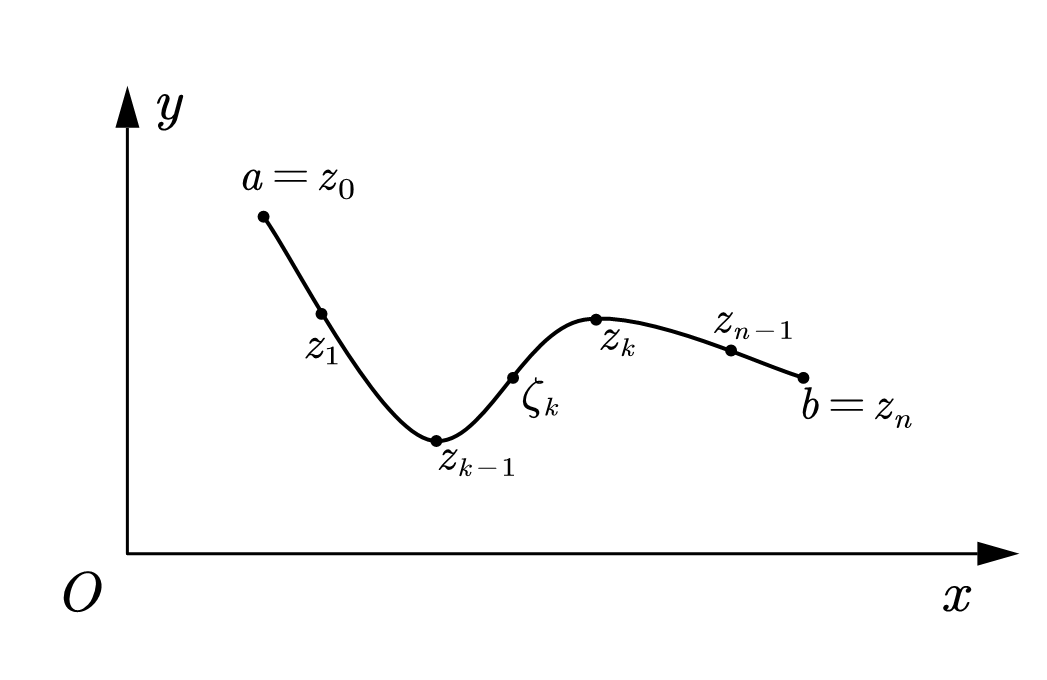
\includegraphics[width=10cm]{./figures/CpxInt_1.png}
\caption{复积分的定义} \label{CpxInt_fig1}
\end{figure}
设$\Delta z_{k}=z_{k}-z_{k-1}$,$\zeta_k$为弧$z_{k-1}z_k$上任意一点,作和$\displaystyle S_{n}=\sum_{k=1}^{n} f\left(\zeta_{k}\right) \Delta z_{k}$.

当分割点的数量无限增加,并且分割$C$所得各个弧段长度中的最大值$d \to 0$时,不论对$C$的分法及$\zeta_k$的取法如何,$S_n$存在极限$S$,则称$ f (z)$沿$C $(从$a$到$b$)可积,称$ S $为$ f (z)$沿$C$(从$a$到$b $)的积分,记作
\begin{equation}
S=\int_{C} f(z) \mathrm{d} z
\end{equation}
其中 $f (z)$称为\textbf{被积函数},$C$称为\textbf{积分路径},而$\displaystyle S=\lim _{n \rightarrow \infty \atop d \rightarrow 0} S_{n}$.
\end{definition}

现在来看一下用定义计算复积分的一个简单例子.
\begin{example}{}
设$C $是一条起点为$a $终点为$b $的逐段光滑曲线,试计算$\displaystyle S=\int_C\mathrm dz$.

用定义来计算该积分.由定义,将$f(z)=1$代入,得:
\begin{equation}
S_{n}=\sum_{k=1}^{n}\left(z_{k}-z_{k-1}\right)=b-a
\end{equation}
所以
\begin{equation}
\int_{C} \mathrm{d} z=\lim _{d \rightarrow 0} S_{n}=b-a
\end{equation}
\end{example}

通过这道例题,我们发现对于函数$f(z)=1$,它的积分值只依赖于积分路径$C$的起点$a$和终点$b$,而与积分路径的形状是无关的.这个性质对于更一般的$f$是否成立?在后面的柯西-古萨定理中,我们将给出答案.

有了积分定义后,最先关心的问题是:积分存在的条件,积分的性质与积分的计算.下面就来讨论这几个问题.

\subsection{复积分存在的一个条件}

为了寻求复变函数积分存在的条件,现在唯一可利用的只有定义.于是问题就归结为考察极限$\displaystyle \lim _{n \rightarrow \infty \atop d \rightarrow 0} S_{n}$的存在条件.为此,不妨将$S_n$变形后再加以考察.

设
\begin{equation}
\begin{array}{l}f(z)=u(x, y)+i v(x, y) \\ \Delta z_{k}=\Delta x_{k}+\mathrm{i} \Delta y_{k} \\ \Delta x_{k}=x_{k}-x_{k-1}, \Delta y_{k}=y_{k}-y_{k-1} \\ \zeta_{k}=\xi_{k}+\mathrm{i} \eta_{k} \\ u_{k}=u\left(\xi_{k}, \eta_{k}\right), v_{k}=v\left(\xi_{k}, \eta_{k}\right)\end{array}
\end{equation}
于是
\begin{equation}
\begin{aligned} \int_{C} f(z) \mathrm{d} z &=\lim _{n \rightarrow \infty \atop d \rightarrow 0} S_{n}=\lim _{n \rightarrow \infty \atop d \rightarrow 0} \sum_{k=1}^{n} f\left(\zeta_{k}\right) \Delta z_{k}=\lim _{n \rightarrow \infty \atop d \rightarrow 0} \sum_{k=1}^{n} f\left(\xi_{k}+\mathrm{i} \eta_{k}\right)\left(\Delta x_{k}+\mathrm{i} \Delta y_{k}\right) \\ &=\lim _{n \rightarrow \infty \atop d \rightarrow 0} \sum_{k=1}^{n}\left[u\left(\xi_{k}, \eta_{k}\right)+\mathrm{i} v\left(\xi_{k}, \eta_{k}\right)\right]\left[\Delta x_{k}+\mathrm{i} \Delta y_{k}\right] \\ &=\lim _{n \rightarrow \infty \atop d \rightarrow 0} \sum_{k=1}^{n}\left(u_{k}+\mathrm{i} v_{k}\right)\left(\Delta x_{k}+\mathrm{i} \Delta y_{k}\right) \\ &=\lim _{n \rightarrow \infty \atop d \rightarrow 0} \sum_{k=1}^{n}\left(u_{k} \Delta x_{k}-v_{k} \Delta y_{k}\right)+\mathrm{i} \lim _{n \rightarrow \infty \atop d \rightarrow 0} \sum_{k=1}^{n}\left(v_{k} \Delta x_{k}-u_{k} \Delta y_{k}\right) \end{aligned}
\end{equation}
由高等数学知道,当$u(x, y)$与$v(x, y)$在$C$上连续时,上式右端两个极限存在,且分别为$\displaystyle \int u \mathrm{d} x-v \mathrm{d} y $与$\displaystyle \int v \mathrm{d} x+u \mathrm{d} y$.

至此,获得积分$\displaystyle \int_{c} f(z) \mathrm{d} z$存在的一个条件是$u(x, y)$与$v(x, y)$均在$C$上连续.而$u(x, y)$与$v(x, y)$在$C$上连续等价于$ f (z)$在$C$上连续,所以,函数$ f (z)$在$C$上连续是积分$\displaystyle \int_{c} f(z) \mathrm{d} z$存在的一个条件.

并且通过上述计算我们还发现了如下定理:
\begin{theorem}{} 
若$ f (z) = u(x, y) + \mathrm iv(x, y)$在曲线$C$上连续,则$f (z)$沿$C$可积,并有
\begin{equation} \label{CpxInt_eq1}
\int_{C} f(z) \mathrm{d} z=\int_{C} u \mathrm{d} x-v \mathrm{d} y+\mathrm{i} \int_{C} v \mathrm{d} x+u \mathrm{d} y
\end{equation}
\end{theorem}

这个积分的重要之处有三:第一,它给出了复变函数积分存在的一个充分条件;第二,它提供了计算复变函数积分的一种方法;其三,\autoref{CpxInt_eq1}表明,研究复变函数的积分问题,可以转化为研究实变量的二元实值函数沿曲线$C $的线积分问题.

\subsection{复积分的性质与计算}

上面我们看到了将线积分和复积分联系起来的\autoref{CpxInt_eq1}.容易想到,线积分的一些性质可移到复变函数的积分上来.

若$ f (z)$与$g (z)$沿曲线$C,C^-$($C^-$表示与曲线$C$方向相反的同一条曲线)可积,则有
\begin{enumerate}
\item \begin{equation}
\int_{C} A f(z) \mathrm{d} z=A \int_{C} f(z) \mathrm{d} z \quad(A \text { 为复常数 })
\end{equation}
\item \begin{equation}
\int_{C}[f(z) \pm g(z)] \mathrm{d} z=\int_{C} f(z) \mathrm{d} z \pm \int_{C} g(z) \mathrm{d} z
\end{equation}
\item \begin{equation} 
\int_{C} f(z) \mathrm{d} z=-\int_{C^{-}} f(z) \mathrm{d} z
\end{equation}
\item \begin{equation}
\int_{C} f(z) \mathrm{d} z=\int_{C_{1}} f(z) \mathrm{d} z+\int_{C_{2}} f(z) \mathrm{d} z\left(C\text{由} C_{1} \text { 与 } C_{2} \text { 首尾相接而成 }\right)
\end{equation}
\item 设$ L$为曲线$C$的长度,若$ f (z)$沿$C$可积,且在$C$上满足$ f (z) \leqslant M $,则
\begin{equation} \label{CpxInt_eq2}
\left|\int_{c} f(z) \mathrm{d} z\right| \leqslant \int_{c}|f(z)| \mathrm{d} s \leqslant M L
\end{equation}
\end{enumerate}

\autoref{CpxInt_eq2}提供了一种估计复变函数积分的模的方法.

到现在为止,计算复变函数积分只有两种方法,一是定义,二是\autoref{CpxInt_eq1}.有无其他方法呢?

我们注意到,由于积分路径常取光滑曲线(或逐段光滑曲线),所以$ f (z) $沿曲线$C $的积分可归结为$f [z(t)]$关于曲线$C$的参数的积分.

事实上,若$C$为光滑曲线(或逐段光滑曲线)
\begin{equation}
\begin{aligned} z &=z(t) \\ &=x(t)+\mathrm{i} y(t),(\alpha \leqslant t \leqslant \beta) \end{aligned}
\end{equation}
则$z^\prime(t)$在$[\alpha, \beta]$上连续,且$z^\prime(t) = x^\prime(t) + \mathrm iy^\prime(t) \neq  0$.再设$ f (z)$在$C$上连续及
\begin{equation}
\begin{aligned} f[z(t)] &=u[x(t), y(t)]+\mathrm{i} v[x(t), y(t)] \\ &=u_{1}(t)+\mathrm{i} v_{1}(t) \end{aligned}
\end{equation}
则有
\begin{equation} \label{CpxInt_eq3}
\begin{aligned} \int_{C} f(z) \mathrm{d} z &=\int u \mathrm{d} x-v \mathrm{d} y+\mathrm{i} \int_{C} v \mathrm{d} x+u \mathrm{d} y \\ &=\int_{\alpha}^{\beta}\left\{u[x(t), y(t)] x^{\prime}(t)-v[x(t), y(t)] y^{\prime}(t)\right\} \mathrm{d} t+\\ & \mathrm{i} \int_{\alpha}^{\beta}\left\{v[x(t), y(t)] x^{\prime}(t)+u[x(t), y(t)] y^{\prime}(t)\right\} \mathrm{d} t \\ &=\int_{\alpha}^{\beta}\left[u_{1}(t)+\mathrm{i} v_{1}(t)\right]\left[x^{\prime}(t)+\mathrm{i} y^{\prime}(t)\right] \mathrm{d} t \\ &=\int_{\alpha}^{\beta} f[z(t)] \mathrm{d} t \end{aligned}
\end{equation}

这样一来,便将$ f (z)$沿曲线$C$的积分归结为$ f (z)$关于曲线$C$的参数$t$的积分.

用\autoref{CpxInt_eq3}来计算积分$\displaystyle \int_{C} f(z) \mathrm{d} z$包含三个步骤:
\begin{enumerate}
\item 写出曲线$C$的方程$z=z(t)=x(t)+i y(t), \alpha \leqslant t \leqslant \beta$
\item 将$ z = z(t)$与$\mathrm{d}z = z^\prime (t)\mathrm{d}t $代入所求积分$\displaystyle \int_{c} f(z) \mathrm{d} z$中
\item 计算\autoref{CpxInt_eq3}右端的关于参数$t$的积分.
\end{enumerate}

有了上述求复变函数的积分的方法之后,我们一起来看几个例子,并尝试用不同的方法来求解.
\begin{example}{}
计算$\displaystyle \int _ C z \mathrm dz$,其中$C$为起点在$a$终点在$b$的一条逐段光滑曲线.

我们用定义来计算一下.

由题知,$f(z)=z$.取$\zeta_k=z_{k-1}$,则$f\left(\zeta_{k}\right)=z_{k-1}$,作和:
\begin{equation}
A_{n}=\sum_{k=1}^{n} f\left(\zeta_{k}\right) \Delta z_{k}=\sum_{k=1}^{n} z_{k-1}\left(z_{k}-z_{k-1}\right)
\end{equation}
因$f(z)=z$在$C$上连续,所以积分一定存在,于是
\begin{equation} \label{CpxInt_eq4}
\int_{C} f(\mathrm{z}) \mathrm{d} \mathrm{z}=\lim _{n \rightarrow \infty \atop d \rightarrow 0} A_{n}
\end{equation}
另外,若取$\zeta_k=z_k$,则$f\left(\zeta_{k}\right)=z_{k}$,作和:
\begin{equation}
B_{n}=\sum_{k=1}^{n} f\left(\zeta_{k}\right) \Delta z_{k}=\sum_{k=1}^{n} z_{k}\left(z_{k}-z_{k-1}\right)
\end{equation}
由之前的讨论知,
\begin{equation}\label{CpxInt_eq5}
\int_{C} f(\mathrm{z}) \mathrm{d} \mathrm{z}=\lim _{n \rightarrow \infty \atop d \rightarrow 0} B_{n}
\end{equation}
由\autoref{CpxInt_eq4}和\autoref{CpxInt_eq5}知,
\begin{equation}
\begin{aligned} \int_{C} f(z) \mathrm{d} z &=\frac{1}{2} \lim _{n \rightarrow \infty \atop d \rightarrow 0}\left(A_{n}+B_{n}\right) \\ &=\frac{1}{2}\left(b^{2}-a^{2}\right) \end{aligned}
\end{equation}
\end{example}
我们再次发现:$f (z) = z$也有一个和$f(z)=1$一样好的性质:它沿曲线$C$的积分只依赖于起点与终点,而与$C $的形状无关!

\begin{example}{} \label{CpxInt_ex1}
试计算$\displaystyle \int_{C} x \mathrm{d} z$,其中$C$为起点在$z = 0$,终点在$z =1+\mathrm i$的直线段.
\begin{figure}[ht]
\centering
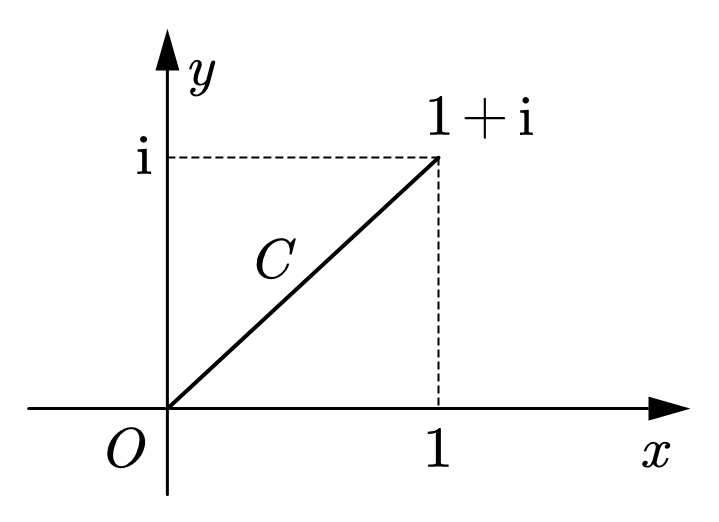
\includegraphics[width=5cm]{./figures/CpxInt_2.png}
\caption{积分路径} \label{CpxInt_fig2}
\end{figure}

我们用\autoref{CpxInt_eq3}计算.首先,写出$C$的方程为
\begin{equation}
z=z(t)=(1+i) t \qquad (0 \leqslant t \leqslant 1)
\end{equation}
由$x+\mathrm{i} y=z=z(t)=(1+\mathrm{i}) t$得$\mathrm{d} z=z^{\prime}(t) \mathrm{d} t=(1+\mathrm{i}) \mathrm{d} t$,将$x=t$和$\mathrm dz$代入所求积分,得
\begin{equation}
\int_{C} x \mathrm{d} z=\int_{0}^{1}(1+\mathrm{i}) t \mathrm{d} t
\end{equation}
最后,计算上式右端的积分得
\begin{equation}
\int_{C} x \mathrm{d} z=\frac{1+\mathrm{i}}{2}
\end{equation}
\end{example}

\begin{example}{} \label{CpxInt_ex2}
设$\Gamma$为由$C_1$与$C_2$首尾相接而成的起点在$z=0$,终点在$ z =1+ \mathrm i $的曲线,如\autoref{CpxInt_fig3}所示.计算$\displaystyle \int_{\Gamma} x \mathrm{d}z$.
\begin{figure}[ht]
\centering
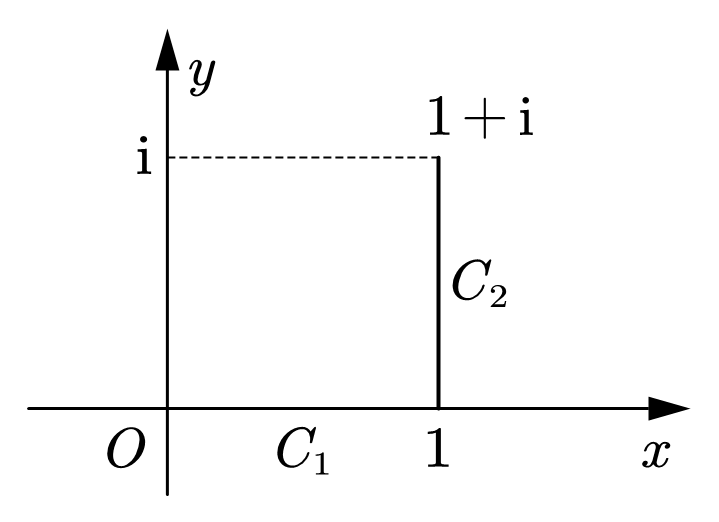
\includegraphics[width=5cm]{./figures/CpxInt_3.png}
\caption{积分路径} \label{CpxInt_fig3}
\end{figure}

首先写出$C_1$和$C_2$的方程为
\begin{equation}
\begin{array}{l}C_{1}: z=z(t)=t(0 \leqslant t \leqslant 1) \\ C_{2}: z=z(t)=1+\text { i }t(0 \leqslant t \leqslant 1)\end{array}
\end{equation}
下面分别计算$C_1$和$C_2$.

在$C_1$上有$x=t, \mathrm{d} z=\mathrm{d} t$,代入$\displaystyle \int_{C_{1}} x \mathrm{d} z$得$\displaystyle \int_{C_{1}} x \mathrm{d} z=\int_{0}^{1} t \mathrm{d} t$.在$C_2$上有$\displaystyle x=\operatorname{Re} z(t)=1, \mathrm{d} z=\mathrm{id} t$,代入$\displaystyle \int_{C_{2}} x \mathrm{d} z$得到$\displaystyle \int_{C_{2}} x \mathrm{d} z=\int_{0}^{1} \mathrm{id} t$.

最后,计算积分得
\begin{equation}
\int_{\Gamma} x \mathrm{d} z=\int_{C_{1}} x \mathrm{d} z+\int_{C_{2}} x \mathrm{d} z=\int_{0}^{1} t \mathrm{d} t+\int_{0}^{1} \mathrm{i} \mathrm{d} t=\frac{1}{2}+\mathrm{i}
\end{equation}
\end{example}

比较\autoref{CpxInt_ex1}和\autoref{CpxInt_ex2},我们发现,对于复变函数$f(z)=x$,积分的结果却与积分路径的选取很有关系.

再来介绍一个十分重要的例题.

\begin{example}{}
试证:
\begin{equation}
\oint_{C} \frac{1}{(z-a)^{n}}=\left\{\begin{array}{ll}2 \pi \mathrm{i}, & n=1 \\ 0, & n \neq 1 \text { 且为整数. }\end{array}\right.
\end{equation}
其中$C$是为以$a $为圆心,以$R $为半径的圆周.

证明:这里的$C $是一条围线,对于沿围线的积分,若无特殊声明,则今后总理解为沿围线的正向积分.

用计算积分的方法来证明本题.

首先,写出$C $的方程为
\begin{equation}
\begin{aligned} z &=z(t) \\ &=a+R \mathrm{e}^{\mathrm{i} \theta} \quad(0 \leqslant \theta \leqslant 2 \pi) \end{aligned}
\end{equation}
其次,$\mathrm{d} z=\mathrm{i} R \mathrm{e}^{\mathrm{i} \theta} \mathrm{d} \theta$,被积函数当$n =1$时为$(z-a)^{-1}=R^{-1} \mathrm{e}^{-\mathrm{i} \theta}$,当$n \ne 1$且为整数时,为$(z-a)^{-n}=R^{-n} \mathrm{e}^{-\mathrm{i} n \theta}$

再次,计算积分,$n=1$时,有
\begin{equation}
\begin{aligned} \oint_{c} \frac{1}{z-a} \mathrm{d} z &=\int_{0}^{2 \pi} \frac{\mathrm{i} R \mathrm{e}^{\mathrm{i} \theta}}{R \mathrm{e}^{\mathrm{i} \theta}} \mathrm{d} \theta \\ &=2 \pi \mathrm{i} \end{aligned}
\end{equation}
当$n \neq 1$且为整数时,有
\begin{equation}
\begin{aligned} \oint_{C} \frac{1}{(z-a)^{n}} \mathrm{d} z &=\int_{0}^{2 \pi} \frac{\mathrm{i} R \mathrm{e}^{\mathrm{i} \theta}}{R^{n} \mathrm{e}^{\mathrm{i} n \theta}} \mathrm{d} \theta \\ &=\frac{\mathrm{i}}{R^{n-1}} \int_{0}^{2 \pi} \mathrm{e}^{-\mathrm{i}(n-1) \theta} \mathrm{d} \theta \\ &=\frac{\mathrm{i}}{R^{n-1}}\left[\int_{0}^{2 \pi} \cos (n-1) \theta \mathrm{d} \theta-\mathrm{i} \int_{0}^{2 \pi} \sin (n-1) \theta \mathrm{d} \theta\right]=0 \end{aligned}
\end{equation}
综上所述,问题得证.
\end{example}

\begin{example}{}
计算积分
\begin{equation}
\oint_{|z-1|=1} \frac{z}{z-1} \mathrm{d} z
\end{equation}
由积分路径为$|z −1|=1$,得$z-1=\mathrm{e}^{\mathrm{i} \theta}(0 \leqslant \theta \leqslant 2 \pi)$.于是,积分路径的方程为
\begin{equation}
z=z(\theta)=1+\mathrm{e}^{\mathrm{i} \theta},(0 \leqslant \theta \leqslant 2 \pi)
\end{equation}
故
\begin{equation}
\begin{aligned} \oint_{z-1} \frac{z}{z-1} \mathrm{d} z &=\int_{0}^{2 \pi} \frac{1+\mathrm{e}^{\mathrm{i} \theta}}{\mathrm{e}^{\mathrm{i} \theta}} \mathrm{ie}^{\mathrm{i} \theta} \mathrm{d} \theta \\ &=\int_{0}^{2 \pi} \mathrm{id} \theta+\int_{0}^{2 \pi}(\cos \theta+\mathrm{i} \sin \theta) \mathrm{d} \theta \\ &=2 \pi \mathrm{i} \end{aligned}
\end{equation}
\end{example}

\begin{example}{}
计算积分
\begin{equation}
\oint_{|z-2|=1} \frac{3 z^{2}}{(z-2)^{3}} \mathrm{d} z
\end{equation}
由$ |z − 2| =1$得积分路径的方程为
\begin{equation}
z=z(\theta)=2+\mathrm{e}^{\mathrm{i} \theta},(0 \leqslant \theta \leqslant 2 \pi)
\end{equation}
于是
\begin{equation}
\begin{aligned} \oint_{|z-2|=1} \frac{3 z^{2}}{(z-2)^{3}} \mathrm{d} z &=\int_{0}^{2 \pi} \frac{3\left(2+\mathrm{e}^{\mathrm{i} \theta}\right)^{2}}{\left(\mathrm{e}^{\mathrm{i} \theta}\right)^{3}} \mathrm{ie}^{\mathrm{i} \theta} \mathrm{d} \theta \\ &=3 \mathrm{i} \int_{0}^{2 \pi}\left(4 \mathrm{e}^{-\mathrm{i} 2 \theta}+4 \mathrm{e}^{\mathrm{i} \theta}+1\right) \mathrm{d} \theta \\ &=6 \pi \mathrm{i} \end{aligned}
\end{equation}
\end{example}